\documentclass[11pt]{amsart}

\usepackage{amsmath}
\usepackage{amssymb}
\usepackage{a4wide}
\usepackage{paralist}
\usepackage{url}
\usepackage{nopageno}
\usepackage{graphicx}

\newcommand{\cA}{\mathcal{A}}
\newcommand{\cS}{\mathcal{S}}
\newcommand{\N}{\mathbb{N}}
\newcommand{\Q}{\mathbb{Q}}
\newcommand{\R}{\mathbb{R}}
\newcommand{\Z}{\mathbb{Z}}

% \numberwithin{equation}{chapter}

\newtheorem{theorem}{\textbf{Theorem}}%%[chapter]
\newtheorem{lemma}[theorem]{Lemma}
\newtheorem{proposition}[theorem]{Proposition}
\newtheorem{corollary}[theorem]{Corollary}
\newtheorem{conj}[theorem]{Conjecture}
\newtheorem{exercise}[theorem]{Exercise}
\newtheorem{example}[theorem]{Example}
\newtheorem{claim}[theorem]{Claim}

\theoremstyle{definition}
\newtheorem{definition}[theorem]{Definition}
\newtheorem{defn}[theorem]{Definition}
\newtheorem{remark}[theorem]{Remark}
\newtheorem{observation}[theorem]{Observation}
\newtheorem{obs}[theorem]{Observation}

\begin{document}

\section{Sheet 2}
\begin{enumerate}

%% EXERCISE 1
\item Show that a face $F$ of a polytope $P$ is exactly the convex hull of all vertices of $P$ contained in~$F$. 
In particular, $P$~has only finitely many faces.

By proposition 2.3, $F$ is a polytope (2.3.i) with $vert(F)=vert(P)\cap F$ (2.3.iii). By proposition 2.2, $F=conv(vert(F))=conv(vert(P)\cap F)$, so we have showed that a face $F$ of a polytope $P$ is exactly the convex hull of all vertices of $P$ contained in ~$F$.

By definition, every polytope $P$ can be written as the convex hull of a finite set of points $V$. By proposition 2.2.ii, $vert(P)\subset V$ for all possible $V$ defining $P$. Since $vert(F)\subset vert(P) \quad\forall F\subset P$ face, and every subset of $vert(P)$ determines at most 1 face, the number of possible faces is bounded by $2^{\#vert(P)}$, which is finite.

%% EXERCISE 2
\item Let $P\subset\R^d$, $Q\subset\R^e$ be two non-empty polytopes. Prove that the set of faces of the cartesian product polytope $P\times Q=\{(p,q)\in\R^{d+e}:p\in P,\; q\in Q\}$ exactly equals $\{F\times G: F\text{ is face of }P, \;G\text{ is face of }Q\}$. Conclude that
\[
    f_k(P\times Q)
    \ = \
    \sum_{%\substack{
      i+j=k,\;i,j\ge0}f_i(P) f_j(Q)
    \qquad
    \text{for } k\ge0.
\]

Let us show that $F\times G$ is a face of $P\times Q$, where $F$ and $G$ are faces of $P$ and $Q$, respectively. Write \[
\begin{array}{c}
 F=\left\{y\in\R^d:ay=b\right\}\cap P\text{, where } a\in(\R^d)^*, b\in\R \text{ and }P\subset\left\{y\in\R^d:ay\leq b\right\}\\
 G=\left\{z\in\R^e:cz=d\right\}\cap Q\text{, where } c\in(\R^e)^*, d\in\R \text{ and }Q\subset\left\{z\in\R^e:cz\leq d\right\}
\end{array}
\]

Note that \[
\begin{split}
F\times G=\left\{\left(\begin{array}{c}
                 y \\ z
                \end{array}
\right)\in\R^{d+e}:ay=b, \quad cz=d, \quad y\in P, \quad z\in Q\right\} \subset \\
\subset \left\{\left(\begin{array}{c}
                 y \\ z
                \end{array}\right)
\in\R^{d+e}:(a,c)
                   \left(\begin{array}{c}
		      y \\ z
		  \end{array}\right)
=b+d \quad y\in P, \quad z\in Q\right\}
\end{split}\]

so $F\times G$ is a face of $P\times Q$ if, and only if, $(a,c)
                   \left(\begin{array}{c}
		      y \\ z
		  \end{array}\right)
\leq b+d \quad \forall y\in P, z\in Q$ and the inclusion can be turned into an equality.

It is easy to see that $(a,c)
                   \left(\begin{array}{c}
		      y \\ z
		  \end{array}\right)
\leq b+d \quad \forall y\in P, z\in Q$, since $ay\leq b \quad \forall y\in P$ and $cz\leq d \quad \forall z\in Q$ by hypothesis.

About the inclusion, a priori we cannot ensure that it is an equality, since there could exist, $y,z$ such that $ay=\tilde b, cz=\tilde d$, with $\tilde b + \tilde d = b+d$.

However, suppose $\tilde b > b$. Then we would have $y\in P$, with $ay > b$, which is a contradiction. So $\tilde b \leq b$. Analogously, $\tilde d \leq d$. Thus, $\tilde b = b$ and $\tilde d = d$, so the inclusion is actually an equality and $F\times G$ is a face of $P\times Q$.
\bigskip

On the other hand, let us show that any face $H$ of $P\times Q$ is the product of a face $F\subset P$ times a face $G\subset Q$.

Since $H$ is a face of $P\times Q$,
\[
H=\left\{
x\in\R^{d+e}:ax=b
\right\}\cap (P\times Q)
\]
for some $a\in\left(\R^{d+e}\right)^*, b\in\R$ with $P\times Q\subset \{ax\leq b\}$.

Write $a=(a_P,a_Q)$, with $a_P\in(\R^d)^*, a_Q\in(\R^e)^*$. Consider the hyperplane of $\R^d$ defined by the equation $\{a_Py=b_P\}$, being $b_P$ such that $P\subset\{a_P y\leq b_P\}$ and $F:=P\cap \{a_Py=b_P\} \neq \varnothing$. Such $b_P$ exists: imagine the hyperplane defined by $a_Py$ swipping from the \emph{valid} side of the infinity until it hits some point of $P$, defining a face $F$ of $P$.

Now let $G=\{z\in\R^e : a_Qz=b-b_P\}\cap Q$. It defines a face of $Q$, because:
\[
\left.\begin{array}{l}
  ax\leq b \Leftrightarrow a_Py+a_Qz\leq b_P+b-b_P \\
  a_Py\leq b_P
\end{array}\right\}\Longrightarrow
a_Qz\leq b-b_P
\]

And we have proved that $H=F\times Q$.
\bigskip

Finally,
\begin{align*}
  f_k(P\times Q)&=\\
  &=\#\left\{\text{faces } H\neq\varnothing  \text{ of }P\times Q: dim(H)=k\right\}=\\
  &=\#\left\{\text{faces } F\times G:F\neq\varnothing  \text{ face of }P, G\neq\varnothing \text{ face of }Q, dim(F)+dim(G)=k\right\}=\\
  &=\sum_{i+j=k; i,j\geq 0} \#\left\{\text{faces } F \text{ of } P : dim(F)=i\right\}
  \cdot\#\left\{\text{faces } G \text{ of } Q : dim(G)=j\right\}=\\  
  &=\sum_{i+j=k; i,j\geq 0} f_i(P)f_j(Q)
% \end{split}
\end{align*}

%% EXERCISE 3
\item Show that all induced cycles of length $3$, $4$ and $5$ in the graph of a simple $d$-polytope~$P$ are graphs of $2$-faces of $P$.
Conclude that the Petersen graph is not the graph of any polytope of any dimension. (\emph{Hint for $5$-cycles:} First show this for $d=3$. Then prove
that any $5$-cycle in a simple polytope is contained in some $3$-face,
and use that faces of  simple polytopes are simple.)
\end{enumerate}


\obs\label{2edges} Two edges incident to a vertex in a graph of a simple polytope $P$ define a unique $2$-face of $P$.
\proof Let $e_1, e_2$ be edges indicent to a vertex $v$. Since $P$ is simple, $v$ can be seen as the intersection of $d$ facets, and both $e_1$ and $e_2$ are the intersection of $d-1$ of these facets. Thus, $e_1$ and $e_2$ share \emph{exactly} $d-2$ facets. 
The intersection of these $d-2$ facets is, by proposition 2.3.ii, a face $F$. Since $e_1,e_2\in F$, $\dim F \geq 2$. On the other hand, $\dim F \leq 2$, because $F$ is the intersection of, at most, $d-\dim F$ facets.$\Box$
\bigskip

% 3-cycles
Take a $3$-cycle $C_3$ in the graph of a simple $d$-polytope~$P$, $v_1v_2v_3$. Let $e_{12},e_{13},e_{23}$ be the edges of the $C_3$, being $e_{ij}$ the edge between $v_i$ and $v_j$.

By Observation \ref{2edges}, $e_{12}$ and $e_{13}$ are incident to the same vertex $v_1$, so they define a $2$-face $F$. Notice that $v_2\in e_{12}\Rightarrow v_2\in F$. Similarly, $v_3\in F$.

Since $F$ is convex, $\lambda u + (1-\lambda) v \in F \quad\forall u,v\in F, \lambda \in [0,1]$. Therefore, $e_{23}=\left\{\lambda v_2 + (1-\lambda) v_3\right\}_{\lambda\in[0,1]}\subset F$ and the triangle defined by $e_{12},e_{13},e_{23}$ is actually a $2$-face of $P$.
\bigskip

% 4-cycles
Take now a $4$-cycle $C_4=v_1v_2v_3v_4$ in the graph of $P$, using the same notation as before, $e_{ij}$, for its edges.

Using Observation \ref{2edges}, let $F$ be the $2$-face defined by the edges $e_{12}$ and $e_{14}$, incidents to $v_1$, and let $G$ be the $2$-face defined by $e_{23}$ and $e_{34}$, incidents to $v_3$.

By convexity, doing the same argumentation that in the previous case, the segment $s_{24}=\left\{\lambda v_2 + (1-\lambda) v_4\right\}_{\lambda\in[0,1]}$ is contained in both $F$ and $G$. In addition, the intersection of faces is a face, so $F\cap G$ is a face of dimension at least $1$. Since $C_4$ is induced, the segment $s_{24}$ is not in the graph of $P$ and $F\cap G$ needs to be a $2$-face. Therefore, $F=G=F\cap G$ and $C_4$ is its graph.
\bigskip

% 5-cycles
Take a $5$-cycle $C_5$ in the graph of $P$, using the same notation as before.

% \emph{Note: I wanted to prove that any $5$-cycle in a simple polytope is contained in some $3$-face, but I think this is enough}
% 
% para el triángulo
% v1=intersection(ABCDEF...)
% v2=intersection(GBCDEF...)
% v3=intersection(GHCDEF...) no puede ser!!! porque v3 y v1 difieren en dos facets, o sea que:
% v3=intersection(HBCDEF...)
% y v1, v2, v3 \in intersection(BCDEF...), que son d-1 facets. Por simpleness, una misma 1-cara???
% v3=intersection(GACDEF...) y solucionao
% 
% cogemos un tetraedro y el triangulo que forma la base B, 123
% 1=B+12+31
% 2=B+12+23
% 3=B+31+23

\emph{Any $5$-cycle in a simple polytope is contained in some $3$-face}:
Using Observation~\ref{2edges}, let $F$ be the $2$-face defined by the edges $e_{12}$ and $e_{23}$, incidents to $v_2$. Notice that $F \cup e_{34}$ needs to be contained in some (at most) $3$-face $\tilde{F}$, because the edge $e_{34}$ is incident to a vertex $v_3\in F$. Analogously, let $G$ be the $2$-face defined by $e_{45}$ and $e_{51}$, incidents to $v_5$.

By convexity, doing the same argumentation that in the previous cases, the segment $s_{14}=\left\{\lambda v_1 + (1-\lambda) v_4\right\}_{\lambda\in[0,1]}$ is contained in both $\tilde{F}$ and $G$. In addition, the intersection of faces is a face, so $\tilde{F}\cap G$ is a face of dimension at least $1$. Since $C_5$ is induced, the segment $s_{14}$ is not in the graph of $P$ and $\dim \tilde{F}\cap G > 1$ . Hence, $G=\tilde{F}\cap G\subset \tilde{F}$ and $C_5$ is contained in a (at most) $3$-face $\tilde{F}$ of $P$. 
\bigskip

\emph{For $d=3$, $C_5$ is the graph of a $2$-face of $P$}:
Since $d=3$, $G(P)$ is planar. Thus, any cycle subdivides $G(P)$ naturally into two subgraphs: the subgraph which is interior to the cycle, $G_i$, and the subgraph which is exterior to the cycle, $G_e$.

Take any planar embedding of $G(P)$ and assume $C_5$ is not the graph of any $2$-face. Notice that both $G_i$ and $G_e$ are not empty: if one of them were empty, $G(P)$ could be embedded in the sphere in such a way that $C_5$ was at the bottom, with no vertex $\notin C_5$ below it, thus being a $2$-face of $P$.

By Balinsky's Theorem, any $G(P)$ is $3$-connected, so at least $3$ edges must connect both $G_i$ and $G_e$ to $C_5$. Hence, one of the vertices of $C_5$ must have at least $4$ edges incident to it, contradicting simpleness of $P$. Therefore, $C_5$ is the graph of a $2$-face of $P$.

Finally, we can conclude that $C_5$ is the graph of a $2$-face of $P$, for any dimension $d$ of $P$. Indeed, $C_5$ is contained in some $3$-face $\tilde{F}$ of $P$. Since faces of simple polytopes are simple, $\tilde{F}$ is a simple $3$-polytope. Thus, $C_5$ is the graph of a $2$-face of $\tilde{F}\subset P$.
\bigskip

% Let $M$ be a minimal $k$-face with $v_i\in M\quad\forall i=1,\ldots 5$. By simpleness of $P$, $M$ can be seen as the intersection of exactly $d-k$ facets.
% 
% On the other hand, every vertex can be seen as the intersection of exactly $d$ facets, by simpleness of $P$ too. In addition, two adjacent vertices $v_i,v_j\in C_5$ share $d-1$ of their facets: Indeed, $e_{ij}$ is a $1$-face, i.e. the intersection of exactly $d-1$ facets, but both $v_i$ and $v_j$ belong to these $d-1$ facets because $v_i,v_j \in e_{ij}$.
% 
% Let $F_i, G_i, H_i$ be facets and consider the different casuistry. Assume WLOG that the facets that are different are those with the lower indices. Assume also that worst case happens: the changing facet is at a different index every time.
% \begin{align*}
%   v_1 &= F_1 \cap F_2 \cap F_3 \cap F_4 \cap F_5 \cap \cdots \cap F_d \\
%   v_2 &= G_1 \cap F_2 \cap F_3 \cap F_4 \cap F_5 \cap \cdots \cap F_d \\
%   v_3 &= G_1 \cap G_2 \cap F_3 \cap F_4 \cap F_5 \cap \cdots \cap F_d \\
%   v_4 &= G_1 \cap G_2 \cap G_3 \cap F_4 \cap F_5 \cap \cdots \cap F_d \\
%   \cdots
% \end{align*}
% 
% Notice that the different facet for $v_5$ cannot be the fourth, because then there would not be possible way to make it consistent for $v_5$ and $v_1$, that are adjacent.

\begin{enumerate}
\setcounter{enumi}{3}
\item Let $n\in\N$ be an integer and $S$ denote a subset of
  $\{1,2,\dots,\lfloor\frac{n}{2}\rfloor\}$.  
  The \emph{circulant graph} $\Gamma_n(S)$ is the graph whose vertex set is $\Z_n$, and whose edge set is the set of pairs of vertices whose difference lies in $S\cup (-S)$. 

The following figure collects all connected circulant graphs on up to $8$~vertices. Determine the \emph{polytopality range} for as many of these graphs as you can, i.e., the set of integers~$d$ such that the graph in question is the graph of a $d$-dimensional polytope.

% \bigskip
% 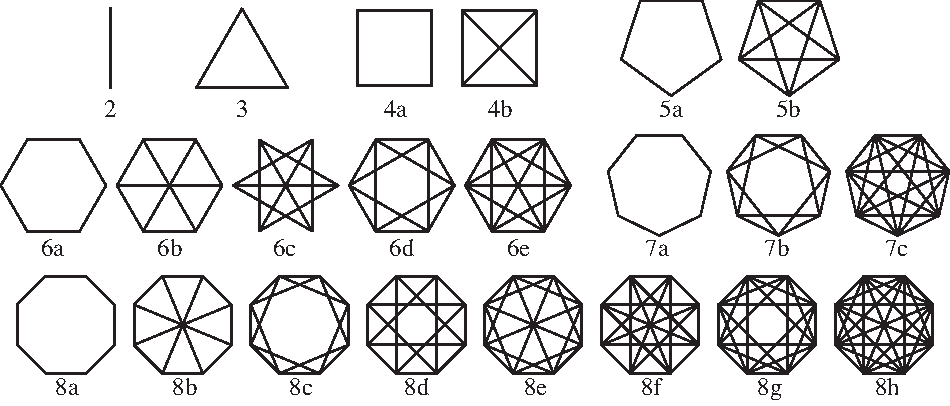
\includegraphics[width=\linewidth]{circulant}

\item Let $\Box^d$ be the $d$-dimensional $\pm1$-cube. How large can the volume of a simplex in $\Box^d$ become? (\emph{Hint:} \url{en.wikipedia.org/wiki/Hadamard_inequality}. Write a  C++ program to attain explicit bounds for $d\ge2$ as large as you can.)
\end{enumerate}

\end{document}





